% Slides for 2024-08-06


\begin{frame}{VOLT Simulation}
    \begin{itemize}
        \item $\sim$400,000 $\rightarrow$ 15,000 Verticies
        \item $\sim$800,000 $\rightarrow$ $\sim$10,000 Faces
        \item $\sim$128 $\rightarrow$ $\sim$12 Objects
        \item Start with solid cylinder
        \item Will need to re-cad 
    \end{itemize}    
\end{frame}

\begin{frame}{Popoto vs Teledyne Testing Plan}
    \centering
    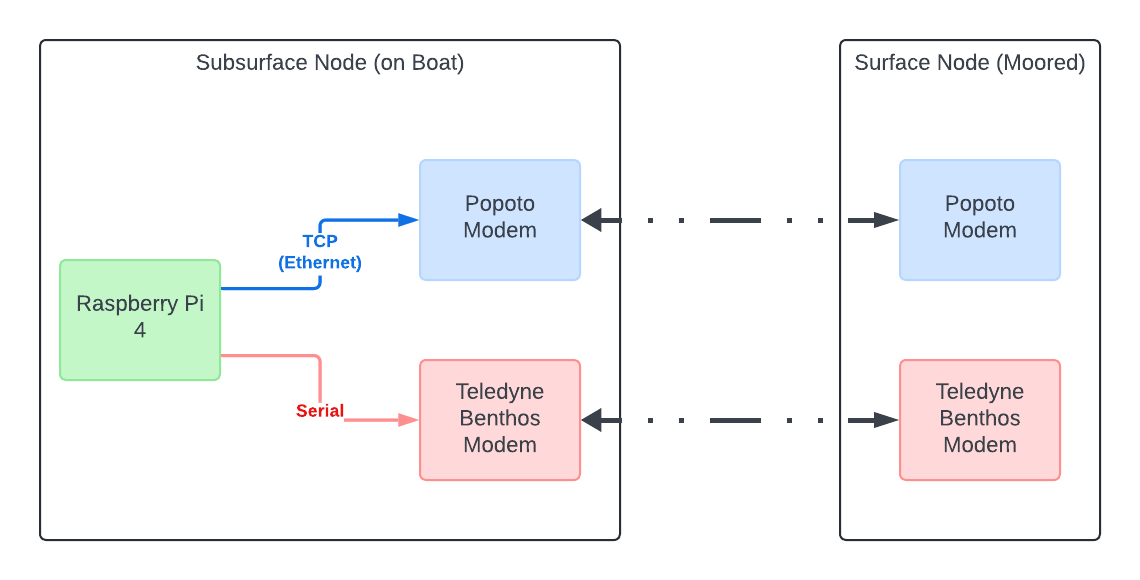
\includegraphics[height=0.7\textheight,width=0.7\textwidth,keepaspectratio]{images/VOLT/VOLT-TestingPlan.png}
\end{frame}



% To create a slide, use the following:
% \begin{frame}{TITLE}
%     BODY
% \end{frame}

% To create a slide with a bullet list, use the following:
% \begin{frame}{TITLE}
%     \begin{itemize}
%         \item ITEM 1
%         \item ITEM 2
%     \end{itemize}    
% \end{frame}

% To create a slide with numbered list, use the following:
% \begin{frame}{TITLE}
%     \begin{enumerate}
%         \item ITEM 1
%         \item ITEM 2
%     \end{enumerate}
% \end{frame}

% To create a slide with a graphic:
% 1. Add the graphic to this folder (named picture.png)
% 2. Use the following:
% \begin{frame}{TITLE}
%     \centering
%     \includegraphics[height=0.7\textheight,width=0.7\textwidth,keepaspectratio]{picture.png}
% \end{frame}

% To create a slide with two columns, use the following:
% \begin{frame}{TITLE}
%     \begin{columns}
%         \begin{column}{0.5\textwidth}
%             COLUMN 1 BODY
%         \end{column}
%         \begin{column}{0.5\textwidth}
%             COLUMN 2 BODY
%         \end{column}
%     \end{columns}
% \end{frame}
